% $Id: testing.tex 5679 2017-10-13 15:24:08Z mskala $

%
% MSK 008 testing and adjustment instructions
% Copyright (C) 2017  Matthew Skala
%
% This program is free software: you can redistribute it and/or modify
% it under the terms of the GNU General Public License as published by
% the Free Software Foundation, version 3.
%
% This program is distributed in the hope that it will be useful,
% but WITHOUT ANY WARRANTY; without even the implied warranty of
% MERCHANTABILITY or FITNESS FOR A PARTICULAR PURPOSE.  See the
% GNU General Public License for more details.
%
% You should have received a copy of the GNU General Public License
% along with this program.  If not, see <http://www.gnu.org/licenses/>.
%
% Matthew Skala
% https://northcoastsynthesis.com/
% mskala@northcoastsynthesis.com
%
\chapter{Adjustment and testing}

The MSK~008 is designed to produce accurate output voltages, a goal partly
achieved through the use of precision components and partly by adjusting
trimmers to compensate for any remaining inaccuracies.  To perform the
adjustment steps you will need an accurate voltage standard (usually, a
good-quality multimeter) to compare against, and at least one patch cable.

For general troubleshooting and testing, you will also need a suitable power
supply and a multimeter.  An oscilloscope is not required, though optional
testing steps using one will be described.

\section{Short-circuit test}

With no power applied to the module, check for short circuits between the
three power connections on the Board~2 Eurorack power connector.  The two
pins at the bottom, marked with white on the circuit board, are for -12V. 
The two at the other end are for +12V; and the remaining six pins in the
middle are all ground pins.  Check between each pairing of these three
voltages, in both directions (six tests in all).  Ideally, you should use a
multimeter's ``diode test'' range for this; if yours has no such range, use
a low resistance-measuring setting. It should read infinite in the reverse
direction (positive lead to $-$12V and negative lead to each of the other
two, as well as positive lead to ground and negative to $+$12V) and greater
than 1V or 1k$\Omega$ in the forward direction (reverse those three
tests).  If any of these six measurements is less than 1k$\Omega$ or 1V,
then something is wrong with the build, most likely a blob of solder
shorting between two connections, and you should troubleshoot that before
applying power.

\emph{Optional}:  Although we test all cables before we sell them, bad
cables have been known to exist, so it might be worth plugging the Eurorack
power cable into the module and repeating these continuity tests across the
cable's corresponding contacts (using bits of narrow-guage wire to get into
the contacts on the cable if necessary) to make sure there are no shorts in
the cable crimping.  Doing this \emph{with the cable connected to the
module} makes it easier to avoid mistakes, because the module itself will
short together all wires that carry equal potential, making it easier to be
sure of testing the relevant adjacent-wire pairs in the cable.

Plug the module into a Eurorack power supply and make sure
neither it nor the power supply emits smoke, overheats, makes any unusual
noises, or smells bad.  If any of those things happen, turn off the power
immediately, and troubleshoot the problem before proceeding.

\emph{Optional}: Plug the module into a Eurorack power supply
\emph{backwards}, see that nothing bad happens, and congratulate yourself on
having assembled the reverse-connection protective circuit properly. 
Reconnect it right way round before proceeding to the next step.

\section{Blinking lights}

Plug the module into a Eurorack power supply, look at the lights on the
front, and flip the switches.  With a channel's switch down ($-$1 position)
the light for that channel should be green; with it up ($+$1 position), the
light should be red; and with it in the middle (0), the light should be
unilluminated.

\section{Output voltage adjustment}

Identify the three trimmers on the back of the module (Board~2).  The basic
concept here is that each channel has five output voltages from $-$2V to
$+$2V.  There is a trimmer (R27 for the left channel and R32 for the right)
which controls the level of the $-$2V output voltage separately per channel. 
Then there is also a third trimmer (R3) which adjusts the spacing between
the steps, for both channels; as a result its effect is greatest on the
$+$2V levels.  Nonetheless we will do the finest adjustments on these
trimmers by examining the $-$1V and $+$1V levels, because those are easier
to generate and test (given that $\pm$2V is full scale on many multimeters)
and choosing points nearer the middle helps distribute residual errors.

\noindent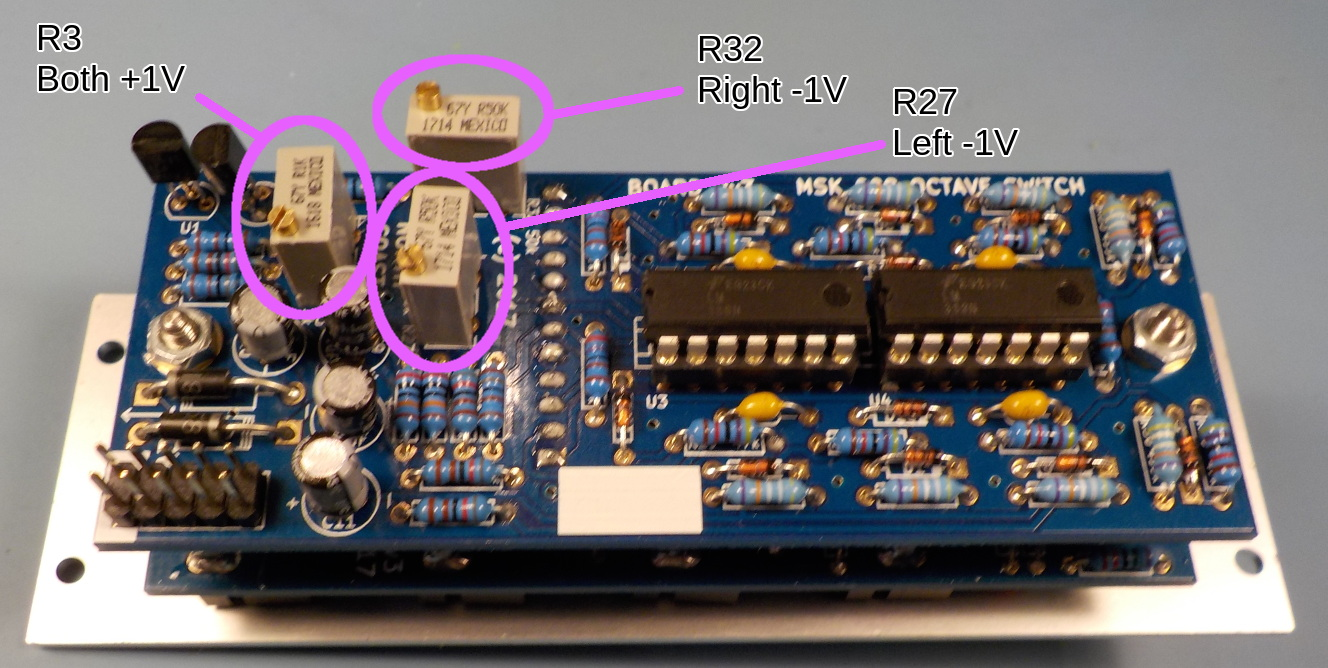
\includegraphics[width=\linewidth]{trimmer-ids.jpg}

For this adjustment procedure you will need to apply power to the module,
and check the output voltages on the two channels under different switch
settings.  If you have a spare 3.5mm jack socket it may be convenient to
make a little adapter for testing the voltage on an output jack using the
socket, a patch cable, and clip-on multimeter probes.  Otherwise, you can
just press the probes against the bare end of a patch cable, or use
alligator clips or similar.  Attempting to probe into the back of Board~1
with pointed probes will probably work, but may be annoying and fiddly.

\textit{Step 1:}  First you will adjust R27 on the $-$2V output of the left
channel.  Patch the output of
the right channel into the quantizer input of the left channel, and switch
both toggle switches to the $-$1 position (both LEDs should glow green). 
Measure the output voltage of the left channel and adjust R27 to bring it
close to $-$2V.  Perfection is not necessary here.  You will be adjusting it
again later; but getting it nearly right at this stage will make the later
adjustments, which interact, much easier.

\noindent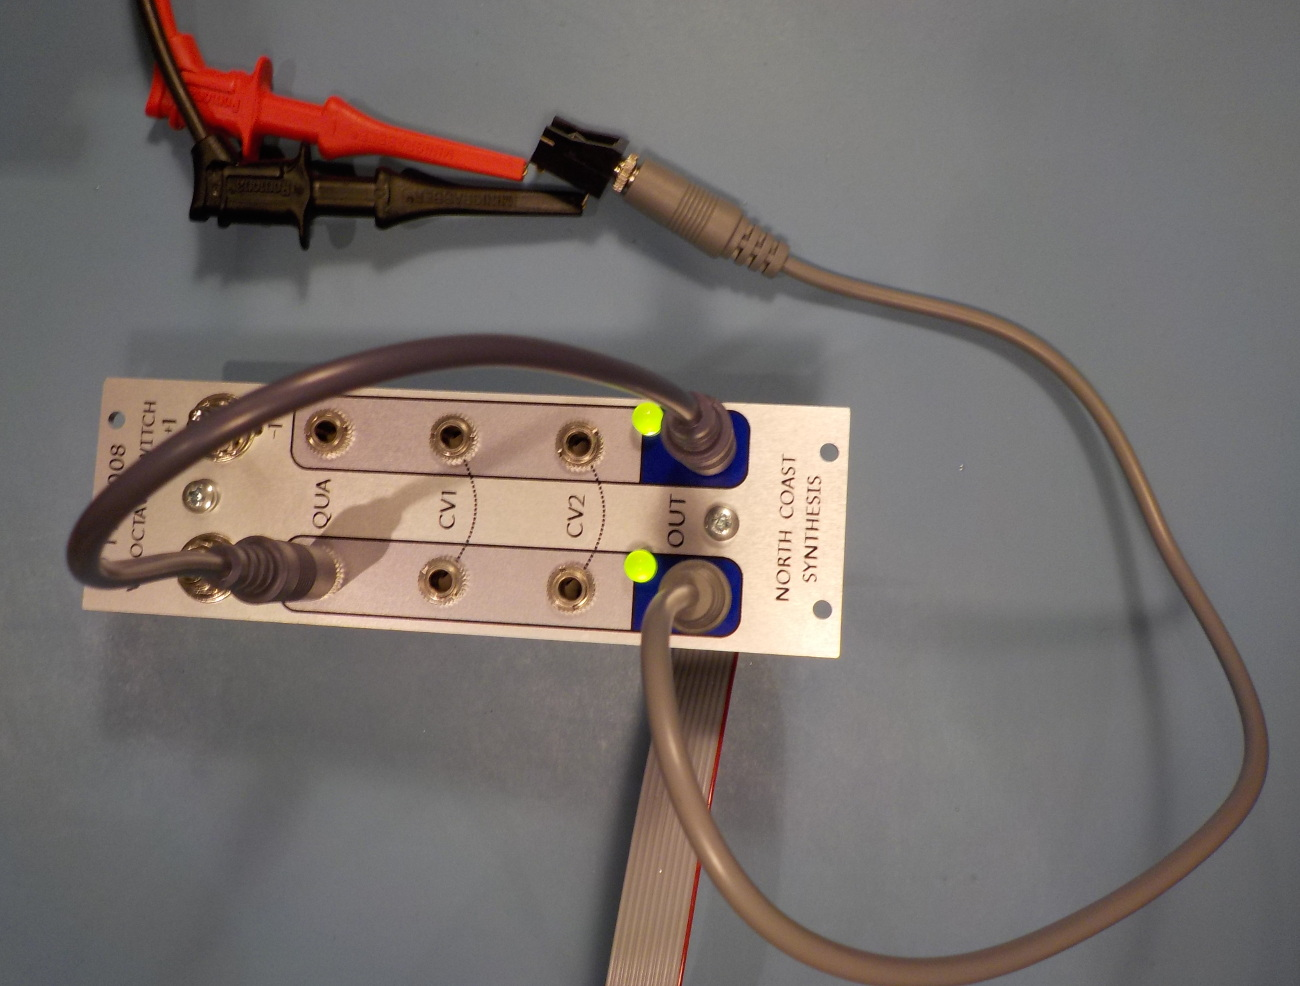
\includegraphics[width=\linewidth]{test-patch.jpg}

\textit{Step 2:}  Switch both toggle switches to the $+$1 position (both
LEDs should glow red).  Measure the output voltage of the left channel and
adjust R3 to bring it close to $+$2V.

\textit{Step 3:}  Reverse the patch:  output of left channel into QUA input
of right channel, voltmeter to measure output of right channel.  Switch both
toggle switches to $-$1, and adjust R32 to bring it close to $-$2V. 
\emph{Then remove the patch cable between the two channels.}

\textit{Step 4:}  Measure the output of the left channel.  Switch its toggle
switch to $-$1, and adjust R27 to bring its output as close to $-$1.000V as
possible.

\textit{Step 5:}  Switch the left channel toggle switch to $+$1, and adjust
R3 to bring its output voltage as close to $+$1.000V as possible.

\textit{Step 6:}  Connect the voltmeter to the right channel.  Set the right
channel's toggle switch to $-$1, and adjust R32 to bring its output voltage
as close to $-$1.000V as possible.

\textit{Step 7:}  Repeat steps 4, 5, and 6 a second time.

Completing these steps as described should be enough to get all the quantizer
output voltages as accurate as the components and your test equipment allow.
Without guarantee, this will normally be better than $\pm$1mV on
all the output voltages.  If you have a lot of patience, you can attempt to
split any remaining error on R3 between the two channels.

If it seems necessary to turn a trimmer all the way to the end of its range,
and especially if even doing so does not allow you to hit the desired output
voltages, then something is wrong; see the troubleshooting suggestions next
section.

\section{Troubleshooting}

It would require several books to convey all the skills and knowledge useful
in troubleshooting even a simple electronic circuit like this one, but here
are some possible symptoms and some suggestions on diagnosis and treatment.

No response from the module at all; \emph{none} of the lights light up, no
signal on the output.  Most likely a power problem, such as a power cable
plugged in wrong or a short circuit.  It might even be a problem in the
power supply and not the module itself.

Module responds, but not as expected:  first attempt to localize the
problem.  Do signals on the CV1 and CV2 inputs appear correctly at the
output (though possibly with DC shifts, and with inversion on inverting CV2
signals)?  If not, check the summing circuits (U5 and associated components)
on Board~1 for problems.  Do voltages on the QUA inputs result in the
expected quantized voltages on the outputs?  If not, look at the quantizers
on Board~2, involving U3 and U4.  Note U3 detects the positive switching
thresholds for both channels and U4 detects the negative thresholds for both
channels; it is not one channel per chip.

If the quantizer appears to operate at all, but input thresholds or output
voltages seem to be wrong: check the voltages along the R8--R12 string for
the nominal values shown on the schematic, though these may correctly
\emph{not} have exactly the values shown if the adjustment procedure has
modified them to compensate for inaccuracies elsewhere.  They should at
least be close.  Wildly incorrect voltages along this string may indicate
problems with the voltage generator section (see circuit explanation),
including U1, U2, and the components near them on Board~2.  Check for solder
bridges on U1 and U2, with an ohmmeter as well as visually.

If the voltages along the resistor string are correct but the quantizer
output or LED responses are wrong, especially if the chips or LED-associated
components get noticeably hot: check for reversed switching diodes.

General tips for debugging DIP ICs:  make sure for, for each IC, that
\begin{itemize}
  \item it really is the type of IC it's supposed to be, not something else
    (beware of cheap ICs you buy from Chinese sellers on eBay, though the
    ones in this project are common enough in more reputable channels that
    you probably wouldn't have attempted that anyway);
  \item it is plugged in snugly;
  \item all the legs of the chip go nicely into the corresponding holes in
    the socket, with none bent outside or folded up under the chip;
  \item it is plugged in \emph{at all} (forgetting to do so is a surprisingly
    common mistake!);
  \item it is plugged in the right way around, with the Pin 1
    indentation or notch at the top and matching the other clues on the
    board (if this is wrong, the chip is probably destroyed and will need to
    be replaced);
  \item there are no solder bridges on the chip socket, unsoldered pins,
    debris clogging the socket holes, or similar;
  \item its decoupling capacitors (the small ceramic ones) are installed and
    there is nothing wrong with their solder joints; and
  \item in the case of the two LM339 chips, try swapping them and see if that
    makes any difference.
\end{itemize}
